\section{03.05.2018 - Hbase}
\begin{itemize}
\item[-] Erzeugen Sie für Ihr Beispiel 2 Hbase (Shell) Tabellen.
\item[-] Füllen Sie die Tabellen mit einigen Testdaten.
\item[-] (Java API) Erzeugen Sie für Ihr Beispiel zwei Hbase Tabellen.
\item[-] Füllen Sie die Tabellen mit einigen Testdaten.
\item[-] Listen Sie die Tabellen auf.
\end{itemize}
\subsection*{Kurzdarstellung der Aufgabenstellung}
Zum Einstieg in NoSQL Datenbanken sollen in Apache Hbase je zwei Tabellen mittels Shell Interface (a) und java SCRIPT/CODE? (b) erstellt und mit Daten befüllt werden. Weiterhin sollen die angelegten Tabellen in Hbase ausgegeben werden mittels vorgegebenen java SCRIPT/CODE (c)?
\subsection*{Lösung}

\begin{itemize}
\item[-] Oracle VM 4.9 starten

\item[-] Tastatur auf Deutsch stellen mittels Eingabe Befehl in Terminal:
\begin{lstlisting}
setxkbmap -layout de
\end{lstlisting}

\subsubsection*{HBASE}
\item[-] HBASE über folgenden Befehlt im Terminal der VM starten:
\begin{lstlisting}
hbase shell
\end{lstlisting}

\item[-] Anlegen der Tabelle „companies“ mit den attributen „id“ und „property“
\begin{lstlisting}
create 'companies1', 'id', 'property'
\end{lstlisting}

\item[-] Daten in die zuvor angelegte Tabelle „companies1“ schreiben:
\begin{lstlisting}
put 'companies1', 'row1', 'id:HRNR', '162'
put 'companies1', 'row1', 'property:Name', 'Musterfirma'
put 'companies1', 'row1', 'property:Gruendung', '1979'
\end{lstlisting}

\item[-] Tabelle „companies1“ mit geschriebenen Daten ausgeben lassen:
\begin{lstlisting}
get 'companies1', 'row1'

COLUMN                CELL
id:HRNR              timestamp=1529566648268, value=162
property:Gruendung   timestamp=1529566667304, value=1979
property:Name        timestamp=1529566659389, value=Musterfirma
3 row(s) in 0.0400 seconds
\end{lstlisting}

\item[-] Anlegen der Tabelle „products1“ mit den attributen „id“ und „property“
\begin{lstlisting}
 create 'products1', 'id', 'property'
\end{lstlisting}

\item[-] Daten in die zuvor angelegte Tabelle „products1“ schreiben:
\begin{lstlisting}
put 'products1', 'row1', 'id:ISBN10', '3866471769'
put 'products1', 'row1', 'id:ISBN13', '978-3866471764'
put 'products1', 'row1', 'property:Typ', 'Buch'
put 'products1', 'row1', 'property:Titel', 'Krieg und Frieden'
put 'products1', 'row1', 'property:Seitenanzahl', '1536'
\end{lstlisting}

\item[-] Tabelle „products1“ mit geschriebenen Daten ausgeben lassen:
\begin{lstlisting}
get 'products1', 'row1'
COLUMN                CELL
id:ISBN10            timestamp=1529566771386, value=3866471769
id:ISBN13            timestamp=1529566777916, value=978-3866471764
property:Seitenanzah timestamp=1529566805924, value=1536
property:Titel       timestamp=1529566797799, value=Krieg und Frieden
property:Typ         timestamp=1529566790781, value=Buch

5 row(s) in 0.0220 seconds
\end{lstlisting}

\subsubsection*{Mittels Java-API}
In der Oracle VM verifizieren ob HBASE als Service gestartet ist und ggf. starten.
\item[-]Oracle JDeveloper 12c starten und Java Developer auswählen
\item[-]Java Projekt „A0305“ mit gewünschtem Zielpfad anlegen „/usr/tmp/dph/A0305/“
\item[-]Alle Java Klassen zu A0305 durch Rechtsklick auf Projektnamen hinzufügen aus:
Location : usr/lib/hadoop (all Library)
Location : usr/lib/hadoop/lib (all Library)
Location : usr/lib/hbase (all Library)
Location : usr/lib/hbase/lib (all Library)
\item[-] Übernahme und Ausführung der SCRIPTE aus den Materialien (Korrektur: TableDescriptor in HtableDescriptor)

\item[-]Anlegen Tabelle „companies2“ mit Spalten „id“ und „property“
\begin{figure}[!htb]
        \begin{minipage}{1\textwidth}
                \centering
                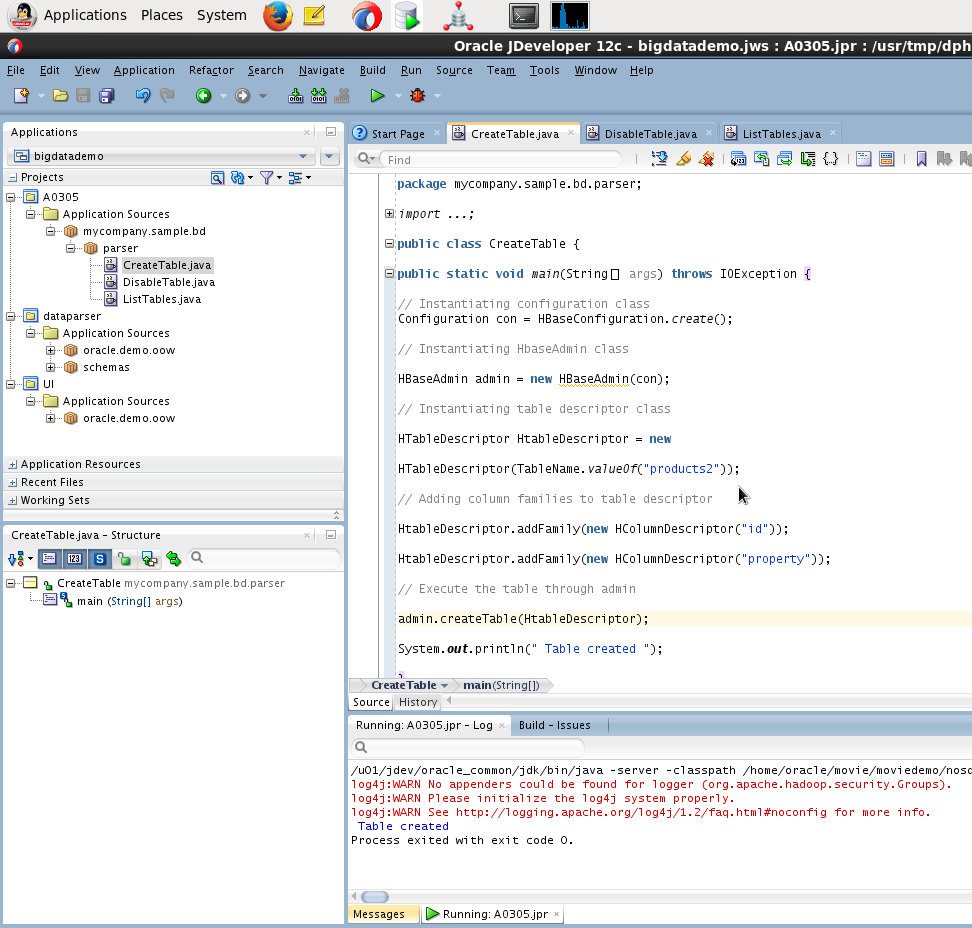
\includegraphics[width=0.90\textwidth]{pics/hbase1.png}\par\vspace{0cm}
                \caption{Tabelle: companies2}
                \label{fig:hbase1}
        \end{minipage}
\end{figure}

\item[-] Anlegen Tabelle „products2“ mit Spalten „id“ und „property“
\begin{figure}[!htb]
        \begin{minipage}{1\textwidth}
                \centering
                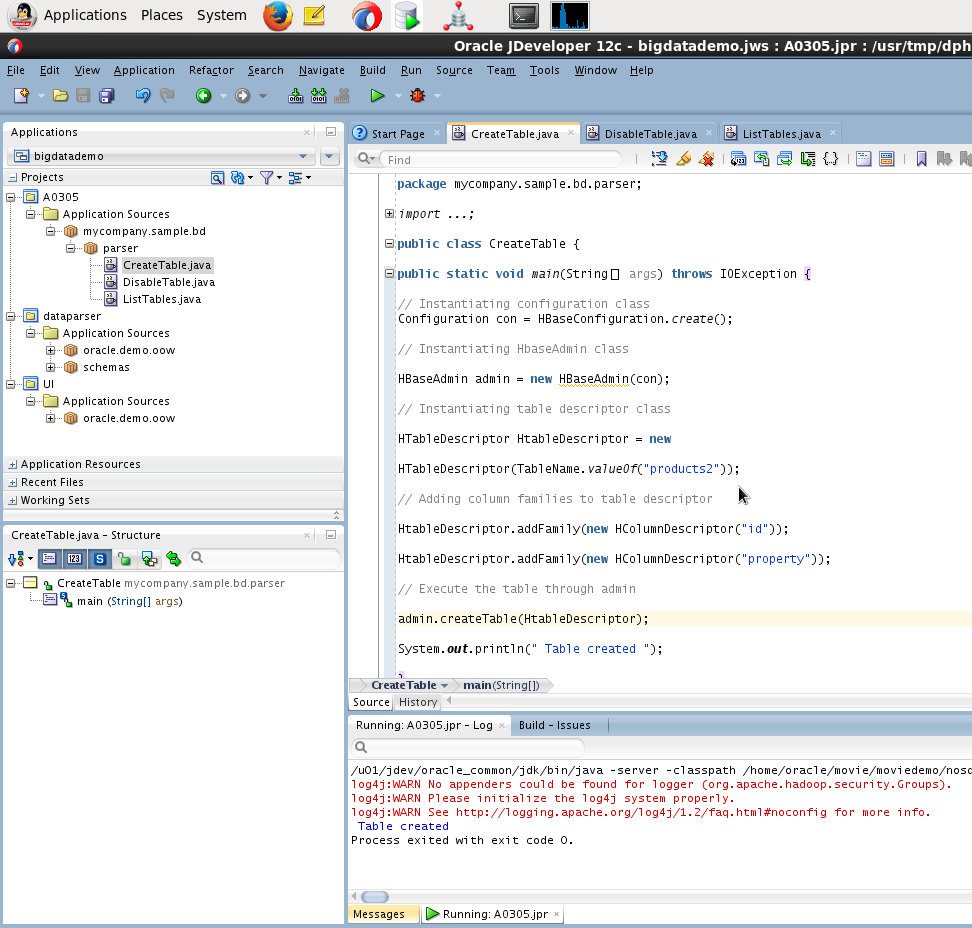
\includegraphics[width=0.90\textwidth]{pics/hbase2.png}\par\vspace{0cm}
                \caption{Tabelle: products2}
                \label{fig:hbase2}
        \end{minipage}
\end{figure}

\item[-] Ausgabe aller angelegten Tabellen in HBASE mittels vorgebenem JAVA code:
\begin{figure}[!htb]
        \begin{minipage}{1\textwidth}
                \centering
                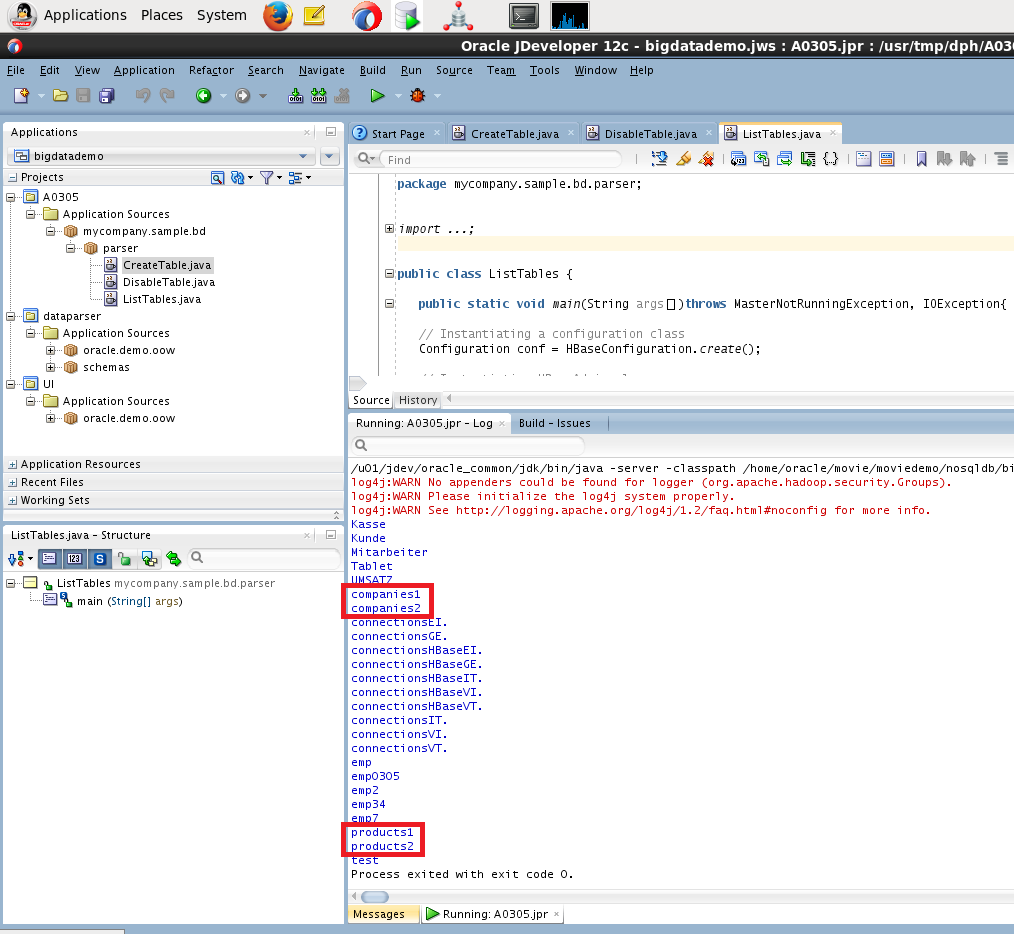
\includegraphics[width=0.90\textwidth]{pics/hbase3.png}\par\vspace{0cm}
                \caption{Ausgabe aller Tabellen}
                \label{fig:hbase3}
        \end{minipage}
\end{figure}

\item[-] Hbase ueber den Terminal der Oracle VM starten:
\begin{lstlisting}
                hbase shell
\end{lstlisting}

\item[-] Daten in die zuvor angelegte Tabelle „companies2“ schreiben:
\begin{lstlisting}
put 'companies2', 'row1', 'id:HRNR', '976'
put 'companies2', 'row1', 'property:Name', 'TheRealDeal'
put 'companies2', 'row1', 'property:Gruender', 'Mr. X'
put 'companies2', 'row1', 'property:Employees', '35'
\end{lstlisting}

\item[-] Tabelle „companies2“ mit geschriebenen Daten ausgeben lassen:
\begin{lstlisting}
get 'companies2', 'row1'
COLUMN                CELL
id:HRNR              timestamp=1529567187758, value=976
property:Employees   timestamp=1529567210676, value=35
property:Gruender    timestamp=1529567203411, value=Mr. X
property:Name        timestamp=1529567196336, value=TheRealDeal
4 row(s) in 0.0290 seconds
\end{lstlisting}

\item[-] Daten in die zuvor angelegte Tabelle „products2“ schreiben:
\begin{lstlisting}
put 'products2', 'row1', 'id:ASIN', 'B015XI6BWE'
put 'products2', 'row1', 'id:Herstellernr', '20B7S1C600'
put 'products2', 'row1', 'id:EAN', '4260444483708'
put 'products2', 'row1', 'property:Typ', 'Laptop'
put 'products2', 'row1', 'property:Model', 'T440'
put 'products2', 'row1', 'property:Marke', 'Think Pad'
0 row(s) in 0.0140 seconds
\end{lstlisting}

\item[-] Tabelle „companies1“ mit geschriebenen Daten ausgeben lassen:
\begin{lstlisting}
get 'products2', 'row1'
COLUMN                CELL
id:ASIN              timestamp=1529567272010, value=B015XI6BWE
id:EAN               timestamp=1529567286841, value=4260444483708
id:Herstellernr      timestamp=1529567279612, value=20B7S1C600
property:Marke       timestamp=1529567306209, value=Think Pad
property:Model       timestamp=1529567299462, value=T440
property:Typ         timestamp=1529567293694, value=Laptop
6 row(s) in 0.0380 seconds
\end{lstlisting}
\end{itemize}
\subsection*{Aufteilung der Aufgaben im Team}
Alle Punkte wurden gemeinsam bearbeitet
\subsection*{Darstellung der benutzen Werkzeuge und Systeme}

\subsubsection*{Entwurfswerkzeug}
Jdeveloper/HBASE
\subsubsection*{Entwicklungsumgebung}
HBASE
